\documentclass[tikz,border=2pt]{standalone}

\usepackage{amsmath} % for \text
\usepackage{xfrac} % for \myfrac
\usepackage{bm} % for \bm
\usetikzlibrary{calc}
\usetikzlibrary{positioning}
\usetikzlibrary{decorations.pathreplacing,decorations.markings}
\usetikzlibrary{patterns} % 加载 patterns 库
\usepackage{comment}


\colorlet{myred}{red!80!black}
\colorlet{myblue}{blue!80!black}
\colorlet{mygreen}{green!60!black}
\colorlet{myorange}{orange!70!red!60!black}
\colorlet{mydarkred}{red!30!black}
\colorlet{mydarkblue}{blue!40!black}
\colorlet{mydarkgreen}{green!30!black}
\colorlet{myred2}{red!50!white}

\colorlet{mylightblue}{blue!60!cyan!80!black!15}
\colorlet{mypurple}{blue!50!red!70}
\colorlet{gaugecol}{red!90!black!70} % Wiki red
\colorlet{leptoncol}{green!80!black!70} % Wiki green
\colorlet{quarkcol}{blue!85!cyan!95!black!55} % Wiki purple
\colorlet{quarkred}{red!98!black!55} % quark red
\colorlet{quarkblue}{blue!85!cyan!98!black!55} % quark blue
\colorlet{quarkgreen}{green!95!black!55} % quark green
\colorlet{gluoncyan}{cyan!100!black!55} % gluon cyan
\colorlet{gluongreen}{green!75!blue!95!black!70} % gluon green
\colorlet{gluonyellow}{yellow!98!black!55} % gluon yellow
\colorlet{gluonorange}{orange!100!black!65} % gluon orange
\colorlet{gluonmagenta}{magenta!100!black!70} % gluon magenta
\colorlet{scalarcol}{yellow!70!orange!98!black}
\colorlet{tensorcol}{blue!50!red!70} % Wiki light blue
\colorlet{groupcol}{orange!15}

\tikzset{
    mynode/.style={
        circle,        % 形状为圆形
        fill=black,    % 填充颜色为黑色
        inner sep=0.4, % 点的大小
        draw           % 添加边框
    }
}


\begin{document}

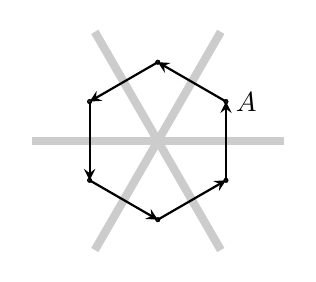
\begin{tikzpicture}[x=2cm, y=2cm]

\newcommand{\radiusA}{0.5}  % 外六边形的半径
\newcommand{\radiusB}{0.8}  % 内六边形的半径
\newcommand{\xShift}{0}   % 六边形的中心 x 偏移
\newcommand{\yShift}{0}   % 六边形的中心 y 偏移

\coordinate (P1) at ([shift=(0:\radiusB)]{\xShift,\yShift});
\coordinate (P2) at ([shift=(60:\radiusB)]{\xShift,\yShift});
\coordinate (P3) at ([shift=(120:\radiusB)]{\xShift,\yShift});
\coordinate (P4) at ([shift=(180:\radiusB)]{\xShift,\yShift});
\coordinate (P5) at ([shift=(240:\radiusB)]{\xShift,\yShift});
\coordinate (P6) at ([shift=(300:\radiusB)]{\xShift,\yShift});

\coordinate (P7) at ([shift=(30:\radiusA)]{\xShift,\yShift});
\coordinate (P8) at ([shift=(90:\radiusA)]{\xShift,\yShift});
\coordinate (P9) at ([shift=(150:\radiusA)]{\xShift,\yShift});
\coordinate (P10) at ([shift=(210:\radiusA)]{\xShift,\yShift});
\coordinate (P11) at ([shift=(270:\radiusA)]{\xShift,\yShift});
\coordinate (P12) at ([shift=(330:\radiusA)]{\xShift,\yShift});


\draw[gray!40, line width=3.0] (P1) -- (P4);
\draw[gray!40, line width=3.0] (P2) -- (P5);
\draw[gray!40, line width=3.0] (P3) -- (P6);

 \fill[ball color=black,scale=1,
      postaction={fill=black,opacity=0.5,
      draw=black!90,ultra thin}] (P7) circle (0.015); 

      \fill[ball color=black,scale=1,
      postaction={fill=black,opacity=0.5,
      draw=black!90,ultra thin}] (P8) circle (0.015); 

      \fill[ball color=black,scale=1,
      postaction={fill=black,opacity=0.5,
      draw=black!90,ultra thin}] (P9) circle (0.015); 

      \fill[ball color=black,scale=1,
      postaction={fill=black,opacity=0.5,
      draw=black!90,ultra thin}] (P10) circle (0.015); 

      \fill[ball color=black,scale=1,
      postaction={fill=black,opacity=0.5,
      draw=black!90,ultra thin}] (P11) circle (0.015); 

      \fill[ball color=black,scale=1,
      postaction={fill=black,opacity=0.5,
      draw=black!90,ultra thin}] (P12) circle (0.015); 

\draw[thick, -stealth] (P7) -- (P8);
\draw[thick, -stealth] (P8) -- (P9);
\draw[thick, -stealth] (P9) -- (P10);
\draw[thick, -stealth] (P10) -- (P11);
\draw[thick, -stealth] (P11) -- (P12);
\draw[thick, -stealth] (P12) -- (P7);

\node[right] at (P7) {$A$};   


\end{tikzpicture}


\end{document}